\clearpage
\graphicspath{{./lib/alice_qkd2/figures/}}
\section{Alice QKD}

\begin{tcolorbox}	
	\begin{tabular}{p{2.75cm} p{0.2cm} p{10.5cm}} 	
        \textbf{Header Files}    &:& alice\_qkd\_*.h \\
		\textbf{Source Files}    &:& alice\_qkd\_*.cpp \\
        \textbf{Version}         &:& 20190410 (Andoni Santos)
	\end{tabular}
\end{tcolorbox}

\maketitle
This block is the main processor for Alice. 

AliceQKD is a superblock intended work as Alice's main processor. It performs a 
series of functions, including classical channel communication with Bob and 
data processing for basis reconciliation, error correction and privacy 
amplification.

\subsection*{Input Signals}

\begin{itemize}
	\item[0] - Binary signal with Alice's key, to be transmitted to Bob.
	\item[1] - Binary signal with Alice's basis, that will be used to encode the key.
	\item[2] - Message signal for receiving incoming messages.
\end{itemize}

\subsection*{Output Signals}

\begin{itemize}
	\item[0] - Binary signal with Alice's key, to be transmitted to Bob.
	\item[1] - Binary signal with Alice's basis, that will be used to encode the key.
	\item[2] - Binary signal with Alice's final key, after the post processing.
	\item[3] - Message signal for sending outgoing messages.
	\item[4] - (Optional) Binary signal with sifted key.
\end{itemize}

% \subsection*{Signals}

% \begin{table}[h]
% 	\centering
% 	\begin{tabular}{|c|l|}
% 		\hline
% 		\textbf{Number of Input Signals} & 3 \\ \hline
%         \textbf{Type of Input Signals} & Binary,
%         Binary,\\
%         & Message\\\hline
%     	\textbf{Number of Output Signals} & 4 (optionally 5) \ \\ \hline
% 		\textbf{Type of Output Signals} & Binary,Binary,Binary,\\
% 		& Message (optional: Binary) \\ \hline
% 	\end{tabular}
% 	\caption{AliceQKD signals}
% 	\label{table:aliceQKD_signals}
% \end{table}

\subsection*{Input Parameters}

\begin{longtable}{|p{25mm}|p{20mm}|p{20mm}|p{20mm}|p{45mm}|}
	\caption*{\textbf{Note:} all the parameters names are only one word. Some of the parameter's names have been split due to space constraints on the table, but their name is the concatenation of multiple lines shown. This may also be true for some default values.}\label{table:aliceQkd_in_par}\\	
	\hline
	\textbf{Parameter} & \textbf{Type} & \textbf{Values} &   \textbf{Default} & \textbf{Description}\\ \hline
	buffSize & unsigned long int & > 0 & 512 & Buffer size for most internal
	signals \\\hline
	maximumEC SyndromeSize & t\_integer & > 0 &  8192 & Buffer size for
	signals where it is important to transmit large quantities of data. \\\hline
	dispBits Interval & t\_integer & > 0 & 50000 & Number of bits transmitted
	before updating the visual interface \\\hline
	folderName & string & valid path & "signals" & Name of the folder where
	signals and output files are saved \\\hline
	reportFile Name & string & valid file name & "alice\_ KeysReport .txt" &
	Name of the file where the overall report for this block is saved
	\\\hline
	toPrint & bool & [true, false] & true & If true, it prints the console
	interface in regular intervals \\\hline
	ipAddress & string & any string & "running locally" & the URL or IP
	address of the remote computer. Only for the purpose of displaying it in the
	interface \\\hline
	photonsPer Pulse & double & any & 0.1 & Average number of photons sent in
	each transmitted pulse. Only for the purpose of displaying it in the
	interface. \\\hline
	% \caption{Error correction input parameters} 
\end{longtable}



\subsection*{Methods}
void initialize(void)
\bigbreak
bool runBlock(void)
\bigbreak
AliceQKD(initializer\_list<Signal *> inputSignals, initializer\_list<Signal *> outputSignals)
\bigbreak
AliceQKD(initializer\_list<Signal*> inputSignals, initializer\_list<Signal*> outputSignals, string sFolderName)
\bigbreak
AliceQKD(initializer\_list<Signal*> inputSignals, initializer\_list<Signal*> outputSignals, t\_integer maxSamplesToProcessAtOnce)
\bigbreak
AliceQKD(initializer\_list<Signal*> inputSignals, initializer\_list<Signal*> outputSignals, string sFolderName, t\_integer maxSamplesToProcessAtOnce)
\bigbreak
AliceQKD(initializer\_list<Signal*> inputSignals, initializer\_list<Signal*> outputSignals, string sFolderName, t\_integer maxSamplesToProcessAtOnce, unsigned long int buffersSize)
\bigbreak
void setErrorCorrectionPartitionSize(t\_integer sz)
\bigbreak
void setErrorCorrectionNumberOfPasses(t\_integer np)
\bigbreak
void setDoublePartitionSize(bool db)
\bigbreak
void setMaximumSyndromeSize(t\_integer mss)
\bigbreak
void setMinimumSyndromeSize(t\_integer minss)
\bigbreak
void setDoubleClickNumber(t\_integer dcn)
\bigbreak
void setNoClickNumber(t\_integer ncn)
\bigbreak
void setBer(t\_real berValue)
\bigbreak
void setSystematicSecurityParameter(t\_integer ssp)
\bigbreak
void setBypassHash(bool bh)
\bigbreak
void setMinimumNumberOfPartitions(t\_integer mnp)
\bigbreak
void setParameterEstimationNumberBits(t\_integer nb)
\bigbreak
void setParameterEstimationNumberBitsToStart(t\_integer nbs)
\bigbreak
void setPrint(bool print)
\bigbreak
void setQberThreshold(const t\_real th)
\bigbreak
void setPhotonsPerPulse(double ppp)
\bigbreak
void setConfidenceInterval(double ci)
\bigbreak
void setIpAddress(string ip)
\bigbreak
string getIpAddress(void)


\subsection*{Functional description}

\begin{figure}[H]
	\centering
	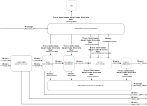
\includegraphics{./lib/alice_qkd2/figures/AliceQKD_blockDiagram.pdf}
\end{figure}

AliceQKD is a superblock intended to do classical channel communication and 
data processing  as required by the BB84 protocol. This superblock requires 
three different inputs:

\begin{itemize}
	\item Messages from Bob, which are used to coordinate the required data 
	processing for key extraction;
	\item A binary signal to be used for the transmitted key;
	\item A binary signal corresponding to the basis which will be used for 
	encoding the data.
\end{itemize}

In addition, this block produces a total of four (or five, optionally) output signals:

\begin{itemize}
	\item	Messages intended to be read by Bob, used to coordinate the required 
	data processing for key extraction;
	\item A binary signal of the data, to be transmitted through the quantum 
	channel;
	\item A binary signal corresponding to the basis which will be used to 
	encoded the transmitted data;
	\item A binary signal with the generated key;
	\item An optional binary signal corresponding to the sifted key.
\end{itemize}


The process inside the superblock is as follows:

The incoming data and basis binary signals are provided as inputs to the 
\textit{AliceIncomingDataProcessor}, together with the 
\textit{transmissionMode} signal. 
The transmission mode controls the behaviour of the 
\textit{AliceIncomingDataProcessor}: it either enables it to continue working 
or tells it to stop reading the input data, while it waits for the current data
to be dispatched.
The data and basis read at the block are sent twice each to the output signals, 
keeping their sync. Each pair of basis and data has a different destination: 
one of the pair is directed to the superblock outputs, in order to transmit the 
data and control the basis for the transmission; and the other pair is sent to 
the \textit{BasisReconciliation} block.

The \textit{BasisReconciliation} block in AliceQKD is configured to responding
to Bobs messages, instead of sending them first. Therefore, it now waits for a 
signal from the 
\textit{MessageProcessorReceiver}. When Bob has enough samples, he should send 
a message containing the basis he used to measure the received data. This 
message is received, identified by its type \texttt{BasisReconciliation1}, and 
interpreted at the \textit{MessageProcessorReceiver}. 
When a message of the correct type arrives, this block sends a signal to the 
\textit{BasisReconciliation} block, containing the list of basis Bob used to 
measure the data on his side. The \textit{BasisReconciliation} block then 
compares the basis received from Bob with the ones that Alice used, and based 
on this it outputs two signals:

\begin{itemize}
	\item A binary evaluation of which basis used 
	by Bob are correct. This is sent to the \textit{MessageProcessorTransmitter}, 
	so that a message can be sent to Bob for him to know which basis were correct.
	\item A binary signal containing the data sent when those basis were used. 
	This is the data that Bob should have measured correctly. This signal is sent 
	to the \textit{ParametersEstimation} block.
\end{itemize} 

The \textit{ParameterEstimation} block receives the key, now free from wrongly
measured bits and from the noClicks and doubleClicks. It accumulates the bits it
receives until it reaches a certain amount, and then waits for an incoming
message from Bob to start processing. The message from Bob contains a seed used
to sample a pseudorandom subset of the accumulated bits, and the value of those
bits that Bob has. Alice compares them to her own bits, and the ratio of correct
bits provides an estimate of the QBER. She then sends her values to Bob, discards
those bits and outputs the QBER value and the remaining bits. The QBER value and
remaining bits are then sent to the \textit{ErrorCorrection} block.

The \textit{ErrorCorrection} block will be responsible for correcting any 
errors that occurred during transmission. Similarly to the 
\textit{BasisReconciliation} block, it is configured to act in response to Bobs 
messages. As such, it waits for data from the 
\textit{MessageProcessorReceiver}, and outputs a response to the 
\textit{MessageProcessorTransmitter}. It also outputs a copy of the 
signal from basis reconciliation, after it has been used for error correction. 
The key output by this block is free from errors, or at least contains a very
small amount of them, depending on the key size and the chosen parameters.

% When the \textit{MessageProcessorReceiver} block receives a message with the type \texttt{ErrorCorrection1}, it starts the Cascade error correction process.
% That message contains the necessary information used in the Cascade process. 
% The explanation of the whole error correction process is somewhat long and not 
% required to understand how the AliceQKD block works. Therefore, further details 
% can be found in the \textit{ErrorCorrection} block's documentation.

After each set of bits is corrected, the data is output to the 
\textit{PrivacyAmplification} block, which does the necessary transformation to 
ensure the information that any attacker might have gained (Eve) is nullified.

The end result, and final output of the superblock, is a secure key 
shared known only to Alice and Bob.

\subsection*{Examples}

\subsection*{Suggestions for future improvement}